%%%%%%%%%%%%%%%%%%%%%%%%%%%%%%%%%%%%%%%%%%%%%%%%%%%%%%%%%%%%%%%%%%%%%
%% This is a (brief) model paper using the achemso class
%% The document class accepts keyval options, which should include
%% the target journal and optionally the manuscript type. 
%%%%%%%%%%%%%%%%%%%%%%%%%%%%%%%%%%%%%%%%%%%%%%%%%%%%%%%%%%%%%%%%%%%%%

%Let's submit to:
%Journal of Medicinal Chemistry will announce a Special Issue on "Artificial Intelligence in Drug Discovery" 

\documentclass[journal=jmcmar,manuscript=article]{achemso}


%%%%%%%%%%%%%%%%%%%%%%%%%%%%%%%%%%%%%%%%%%%%%%%%%%%%%%%%%%%%%%%%%%%%%
%% Place any additional packages needed here.  Only include packages
%% which are essential, to avoid problems later. Do NOT use any
%% packages which require e-TeX (for example etoolbox): the e-TeX
%% extensions are not currently available on the ACS conversion
%% servers.
%%%%%%%%%%%%%%%%%%%%%%%%%%%%%%%%%%%%%%%%%%%%%%%%%%%%%%%%%%%%%%%%%%%%%
\usepackage[version=3]{mhchem} % Formula subscripts using \ce{}
\usepackage{subcaption}
\usepackage{array}
\usepackage{url}
\usepackage{xr-hyper}
\usepackage{hyperref}
\usepackage{multirow}
\usepackage[flushleft]{threeparttable}
\captionsetup[figure]{font=small,labelfont=small}

\makeatletter
\newcommand*{\addFileDependency}[1]{% argument=file name and extension
  \typeout{(#1)}
  \@addtofilelist{#1}
  \IfFileExists{#1}{}{\typeout{No file #1.}}
}
\setlength\acs@tocentry@height{8.25cm}
\setlength\acs@tocentry@width{4.45cm}
\makeatother
\newcommand*{\myexternaldocument}[1]{%
    \externaldocument{#1}%
    \addFileDependency{#1.tex}%
    \addFileDependency{#1.aux}%
}

\myexternaldocument{supp}

%%%%%%%%%%%%%%%%%%%%%%%%%%%%%%%%%%%%%%%%%%%%%%%%%%%%%%%%%%%%%%%%%%%%%
%% If issues arise when submitting your manuscript, you may want to
%% un-comment the next line.  This provides information on the
%% version of every file you have used.
%%%%%%%%%%%%%%%%%%%%%%%%%%%%%%%%%%%%%%%%%%%%%%%%%%%%%%%%%%%%%%%%%%%%%
%%\listfiles

%%%%%%%%%%%%%%%%%%%%%%%%%%%%%%%%%%%%%%%%%%%%%%%%%%%%%%%%%%%%%%%%%%%%%
%% Place any additional macros here.  Please use \newcommand* where
%% possible, and avoid layout-changing macros (which are not used
%% when typesetting).
%%%%%%%%%%%%%%%%%%%%%%%%%%%%%%%%%%%%%%%%%%%%%%%%%%%%%%%%%%%%%%%%%%%%%
\newcommand*\mycommand[1]{\texttt{\emph{#1}}}


%%%%%%%%%%%%%%%%%%%%%%%%%%%%%%%%%%%%%%%%%%%%%%%%%%%%%%%%%%%%%%%%%%%%%
%% Meta-data block
%% ---------------
%% Each author should be given as a separate \author command.
%%
%% Corresponding authors should have an e-mail given after the author
%% name as an \email command. Phone and fax numbers can be given
%% using \phone and \fax, respectively; this information is optional.
%%
%% The affiliation of authors is given after the authors; each
%% \affiliation command applies to all preceding authors not already
%% assigned an affiliation.
%%
%% The affiliation takes an option argument for the short name.  This
%% will typically be something like "University of Somewhere".
%%
%% The \altaffiliation macro should be used for new address, etc.
%% On the other hand, \alsoaffiliation is used on a per author basis
%% when authors are associated with multiple institutions.
%%%%%%%%%%%%%%%%%%%%%%%%%%%%%%%%%%%%%%%%%%%%%%%%%%%%%%%%%%%%%%%%%%%%%
\author{Paul G. Francoeur}
\author{David R. Koes}
\email{dkoes@pitt.edu}
\affiliation[Pitt]{Department of Computational and Systems Biology, University of Pittsburgh, Pittsburgh, PA 15260}


%%%%%%%%%%%%%%%%%%%%%%%%%%%%%%%%%%%%%%%%%%%%%%%%%%%%%%%%%%%%%%%%%%%%%
%% The document title should be given as usual. Some journals require
%% a running title from the author: this should be supplied as an
%% optional argument to \title.
%%%%%%%%%%%%%%%%%%%%%%%%%%%%%%%%%%%%%%%%%%%%%%%%%%%%%%%%%%%%%%%%%%%%%
\title[some shit we did]{Fancy title for Imputation project}

%%%%%%%%%%%%%%%%%%%%%%%%%%%%%%%%%%%%%%%%%%%%%%%%%%%%%%%%%%%%%%%%%%%%%
%% Some journals require a list of abbreviations or keywords to be
%% supplied. These should be set up here, and will be printed after
%% the title and author information, if needed.
%%%%%%%%%%%%%%%%%%%%%%%%%%%%%%%%%%%%%%%%%%%%%%%%%%%%%%%%%%%%%%%%%%%%%
\keywords{structure-based drug design, molecular docking, deep learning, machine learning}

%%%%%%%%%%%%%%%%%%%%%%%%%%%%%%%%%%%%%%%%%%%%%%%%%%%%%%%%%%%%%%%%%%%%%
%% The manuscript does not need to include \maketitle, which is
%% executed automatically.
%%%%%%%%%%%%%%%%%%%%%%%%%%%%%%%%%%%%%%%%%%%%%%%%%%%%%%%%%%%%%%%%%%%%%
\begin{document}

%%%%%%%%%%%%%%%%%%%%%%%%%%%%%%%%%%%%%%%%%%%%%%%%%%%%%%%%%%%%%%%%%%%%%
%% The "tocentry" environment can be used to create an entry for the
%% graphical table of contents. It is given here as some journals
%% require that it is printed as part of the abstract page. It will
%% be automatically moved as appropriate.
%%%%%%%%%%%%%%%%%%%%%%%%%%%%%%%%%%%%%%%%%%%%%%%%%%%%%%%%%%%%%%%%%%%%%
\begin{tocentry}

% Some journals require a graphical entry for the Table of Contents.
% This should be laid out ``print ready'' so that the sizing of the
% text is correct.

% Inside the \texttt{tocentry} environment, the font used is Helvetica
% 8\,pt, as required by \emph{Journal of the American Chemical
% Society}.

% The surrounding frame is 9\,cm by 3.5\,cm, which is the maximum
% permitted for  \emph{Journal of the American Chemical Society}
% graphical table of content entries. The box will not resize if the
% content is too big: instead it will overflow the edge of the box.

% This box and the associated title will always be printed on a
% separate page at the end of the document.
%\includegraphics{figures/TOC_CD2020.pdf}
\end{tocentry}

%%%%%%%%%%%%%%%%%%%%%%%%%%%%%%%%%%%%%%%%%%%%%%%%%%%%%%%%%%%%%%%%%%%%%
%% The abstract environment will automatically gobble the contents
%% if an abstract is not used by the target journal.
%%%%%%%%%%%%%%%%%%%%%%%%%%%%%%%%%%%%%%%%%%%%%%%%%%%%%%%%%%%%%%%%%%%%%
\begin{abstract}
TODO -- last

\end{abstract}

%%%%%%%%%%%%%%%%%%%%%%%%%%%%%%%%%

%%%%%%%%%%%%%%%%%%%%%%%%%%%%%%%%%%%%%%%%%%%%%%%%%%%%%%%%%%%%%%%%%%%%%
%% Introduction and Background
%%%%%%%%%%%%%%%%%%%%%%%%%%%%%%%%%%%%%%%%%%%%%%%%%%%%%%%%%%%%%%%%%%%%%
\section{Introduction}

Part of the recent successes of Deep Learning have been due in part to training very large models on large datasets.
A recent example of this phenomenon in the protein structure prediction task is AlphaFold, which has 93 million parameters, and was trained on the 204,104 structures available in the protein data bank and 355,993 unlabeled sequences from Uniclust30 \cite{alphafold}.
Conversely, for structure based predictions for protein-ligand binding affinity, we are much more data limited.
The most common dataset for model evaluation is the PDBbind, which only contains a maximum of 23,496 entries \cite{pdbbind2016}.
%should there be one more sentence here??

%need to figure out a clean way to transition into the next section talking about the data expansion we did for CD2020.
For structure based ML models, our training data is an order of magnitude smaller.
Clearly, there is a desire to expand the available training data, which in turn can enable the use of models with higher parameter count for this task.
Additionally, since it is both time consuming and expensive to generate both a crystal structure and binding affinity measurement for a given receptor ligand pair, it makes sense to explore \textit{in silica} methods to expand the training data.
In prior work, we introduced the CrossDocked2020 dataset which expands the available binding complexes through crossdocking\cite{crossdocked2020}.
We made the assumption that ligands will bind to similar receptors in order to group the PDB into binding pockets, and combinatorially expand the receptor ligand complexes by docking each ligand in a pocket to each receptor in said pocket.
This increased the number of binding poses from $\sim$200,000 in the PDBbind general set to $\sim$22.5million poses in CrossDocked2020\cite{crossdocked2020}.

However, a shortcoming of this approach is that it does not expand the binding affinity data.
Only $\sim$40\% of CrossDocked2020 has a binding affinity label, since they were taken from the PDBbind general set.
Thus, in terms of binding affinity predictions, models trained on CrossDocked2020 are observing the same distribution of binding affinity training data as models trained on the PDBbind general set.
In this work, we investigate the effect of various imputation strategies for the missing binding affinity labels on model performance.

%Introduce the idea of data imputation here -- probably brief description of the types of imputation & classifications of missingness.
Imputation is the process of replacing missing data with potential or estimated values, with general reviews available on the topic.\cite{surveyReview1, review2}%cite review
There are three general classes of missing data: 1) missing completely at random (MCAR), 2) missing at random (MAR), and 3) missing not at random (MNAR).
The differential between these classes is based on the likelihood of a particular data point being missing.
Data MCAR refers to data where the probability of being missing is independent of the observed and unobserved measurements.
MAR data is the next step, where the probability of a data point being missing is related to the observable data.
Lastly, data MNAR is the hardest case where the probability of missing data depends on both the observed and unobserved values.
Notably, these three categories describe a sort of continuum of categories of missingness, and it is mostly impossible to unambiguously categorize missing data into one of these three types.
Typically, people treat all of the missing data as MAR since this category resides in the middle of the categories.

There are several approaches to imputing the missing data.
The simplest, and easiest, of which is to delete or ignore the missing values.
This was the approach that we utilized in the CrossDocked2020 paper, where the binding affinity loss was only applied to complexes which had a labeled binding affinity.
However, it is known that this approach, while easy, can introduce extra bias into the models, especially if the missing data is not randomly distributed.\cite{rev1support}
The next easiest method of imputation is known as "simple imputation".
It entails replacing the missing values by a single quantifiable attribute of the non-missing values (e.g. mean, median, mode).
Unfortunately, these methods may produce bias or unrealistic results on high-dimensional data sets, which is what we are using in this work. \cite{SICE}

Thus, we turn to regression imputation.
In this form of imputation a model is fit to the known data points and then is used to assign the imputed labels to the missing data.
There are several approaches to this type of imputation, from statistical such as a weighted quantile regression, to more machine learning inspired approaches like k-nearest neighbors, support vector machines, random forests, etc.\cite{rev1support,review2}
ML based imputation approaches have been successful across the medical field, showing promise in imputing Medical Expenditure Panel Surveys\cite{MLimpMedsurvey}, or being utilized in clinical decision making.\cite{MLclinicDecision}.
However, to the best of our knowledge, an ML approach to imputing missing protein-ligand binding affinities has not been studied.

The closest is \citet{peptideMHCimp}, who examined a variety of methods on imputing binding affinities for peptide-Major Histocompatibility Complex interactions.
Notably the approaches utilized in this paper were not ML based, and were about predicting a singular class of binding affinity interactions between the MHC class of receptors and their peptide substrates.\cite{peptideMHCimp}
This is similar, but not exactly our need, which is to have a model that predicts binding affinities for any receptor and small molecule ligand.
The most common ML models employed in imputation are k-nearest neighbor (k-NN) models and random forest models.\cite{review2}
k-NN models are tricky to fit to our molecular data, as our CNN based models and molecular grids do not have a good input representation for our receptor-ligand complexes amenable to a distancing metric.
Additionally, \citet{graphEditDist} show that fingerprint based similarity metrics can incorrectly measure the similarity between molecules, and suggest a similarity based on graph edit distance.
However, for our large dataset, there is considerable computational expense in computing these similarity metrics. 
We also know that our CNN-based models perform similarly to other random forest based methods on predicting protein-ligand binding affinity.\cite{crossdocked2020}
Thus, we investigate using our CNN model architecture and an ensemble of these CNN models to impute the missing binding affinities in this work.

%%%%%%%%%%%%%%%%%%%%%%%%%%%%%%%%%%%%%%%%%%%%%%%%%%%%%%%%%%%%%%%%%%%%%
%% Methods
%%%%%%%%%%%%%%%%%%%%%%%%%%%%%%%%%%%%%%%%%%%%%%%%%%%%%%%%%%%%%%%%%%%%%
\section{Methods}
Here we describe our 3D grid based CNN model architecture, the dataset we are utilizing for our experiments, and the training procedure utilized for each of the experiments.

\subsection{Model Architecture}
We are utilizing the Def2018 model previously described.\cite{crossdocked2020}
Briefly, it is a convolutional neural network consisting of a 2x2x2 average pool, followed by a 3x3x3 convolution and ReLU, followed by a 1x1x1 convolution and ReLU layer. 
This pool-convolution-convolution block is repeated 1 time, and then followed by a final 2x2x2 average pool and 3x3x3 convolution plus ReLU layer.
The convolution process results in a total of 6x6x6x128 features which are passed to the two output fully connected layers.
These output layers predict the binding affinity and pose score respectively, and share weights.
The input to our model is a 24x24x24angstrom grid at 0.5angstrom resolution of a continuous Gaussian density of 14 ligand and 14 receptor atom types.
These grids are generated on the fly by \texttt{libmolgrid}.\cite{sunseri2019libmolgrid}

\subsection{Dataset}%TODO -- Get the NUMBERS and PERCENTAGE below.
Similarly we are utilizing the CrossDocked2020v1.3 dataset, following the same clustered cross validation splits utilized in the CrossDocked2020 publication.\cite{crossdocked2020}
CrossDocked2020v1.3 contains NUMBER of binding pockets, consisting of NUMBER pocket:ligand pairs, and a total of NUMBER poses.
As previously mentioned, PERCENTAGE of binding poses have labeled binding affinity data.
The dataset was generated by docking ligands for a given receptor into other receptors in the same pocket, as defined by Pocketome\cite{pocketome}.
We label poses as good if their root mean square deviation (RMSD) of the docked pose to the crystal pose is less than 2, or bad otherwise.
If a given ligand has binding affinity data in the PDBBind version 2017, we assume that it would have the same binding affinity label for all members of a pocket.
This data was clustered using the ProBiS \cite{ProBiS} algorithm with the z-score parameter set to 3.5.
Each cluster was then randomly assigned to one of 3 folds for clustered cross-validation.


\subsection{Model Training Procedure}
Consistent with our prior work\cite{crossdocked2020}, models were trained using our custom fork of the Caffe deep learning framework \cite{jia2014caffe} with \texttt{libmolgrid} integration \cite{sunseri2019libmolgrid} using the \texttt{train.py} script available at \url{https://github.com/gnina/scripts}.
Training examples were randomly shuffled with 50 examples being provided in the training batch.
Batches were balanced with respect to class labels (low RMSD vs high RMSD poses) and examples were stratified with respect to the receptor so that targets are sampled uniformly during training.
The structures were also randomly rotated and translated up to 6{\AA}.
We utilized the stochasitc gradient descent (SGD) optimizer with an initial learning rate of 0.01 and momentum of 0.9 with weight decay of 0.001.

Lastly, we utilized early stopping to terminate training.
We monitor performance on a reduced version of the training set and testing set, containing about 200,000 complexes for training.
This was generated automatically by the \texttt{train.py} script with the \textit{percent\_reduced} parameter set to 0.132.
Every 1000 training iterations, we evaluate the reduced set.
If the performance ceases to improve over 200 evaluations (\textit{step\_when}), we lower the learning rate by a factor of 10.
The learning rate is allowed to lower 3 times (\textit{step\_end\_cnt}), after which training will cease.

\subsection{Experimental Setup}
For each of the following experiments we train 5 models, each utilizing a different random seed, on the 3-fold clustered cross-validation splits previously described.

The general schema of each experiment is: 1) Train and evaluate an initial model on the data with missing labels, 2) Use the trained model and an imputation scheme to impute the missing labels, 3) Train and evaluate a new model on the imputed data, 4) Repeat 2-3 until performance on the test set stops.
We investigated several imputation schemes in order to determine their effect on model performance on binding affinity prediction.
First, we utilized the simplest approach: treating each binding pose as a different example and simply utilizing the predictions of a trained model independently.
That is, there was no ensemble between the different seeds on the imputation for the missing data.
This results in each seeded model having a different training set from one another.

The second approach was to utilize the mean of each of the 5 models to produce the imputation label for each pose.
This allows for the same training set to be utilized for each seed during training at each round of imputation.
However, this approach also results in each binding pose for a given pocket-ligand complex to have a different binding affinity label during the next round of training.
Notably, this results in only the imputed binding affinities having a pose-specific label for the binding affinity, unlike the rest of the training data.
It is unclear whether this is desirable or not, so we also investigated a third imputation approach.

For the third imputation approach, for each pocket-ligand complex we stored the predicted label of every pose.
We then took as our imputation the max, median, or minimum of these predicted values as the label for every pose for said pocket-ligand complex.
In contrast to the second imputation scheme, this approach results in a singular value being utilized for every pose.

A potential flaw with the third imputation approach is that we also include the predicted binding affinity for poses which we know are not in the correct binding orientation.
%Question -- numbers for what I say below?
This could cause potential confusion during model training as these predictions from poor quality poses (which make up the vast majority of the poses in our data set) have a significant impact on the median and min selection of the list we generate per pocket-ligand complex in approach 3.
Thus we also investigate if generating this last has a beneficial effect when we only include predictions from poses which are labeled good (less than 2 RMSD from the native crystal pose).

Lastly, we characterize how much imputed data is necessary to achieve the performance gain for our fourth imputation method.
We evaluate randomly adding increments of 20 percent of the imputed binding labels to the training data of the model.
E.G. training with no imputed labels, 20, 40, 60, 80, or 100 percent of the imputed labels.
This allows us to characterize the effect of adding various levels of imputed data to the training of our models.

In order to compare between these experiments We adopt the same testing criteria and methods described in the initial CrossDocked2020 paper\cite{crossdocked2020}.
Namely, that for each pocket-ligand pair we select a singular pose by selecting the pose with the highest predicted pose score to be our candidate. 
We then calculate the Pearson's $R$ and the root mean squared error (RMSE) between the candidate poses binding affinity labels and the predictions from our model.
When calculating this, we only evaluate the molecules in the test set which have a binding affinity label.
We additionally evaluate the area under the receiver operating characteristic curve (AUC), and the fraction of times that the top ranked binding pose is less than 2 RMSD to the native crystal pose (Top1) to serve as measures of our model's ability to distinguish bad and good poses.

%TODO -- make a series of figures for each of the expiermental setups & referemce them to these sections

%%%%%%%%%%%%%%%%%%%%%%%%%%%%%%%%%%%%%%%%%%%%%%%%%%%%%%%%%%%%%%%%%%%%%
%% Results
%%%%%%%%%%%%%%%%%%%%%%%%%%%%%%%%%%%%%%%%%%%%%%%%%%%%%%%%%%%%%%%%%%%%%
\section{Results}

\begin{figure}[tbph]
    \centering
    \begin{subfigure}[t]{0.48\textwidth}
        \centering
        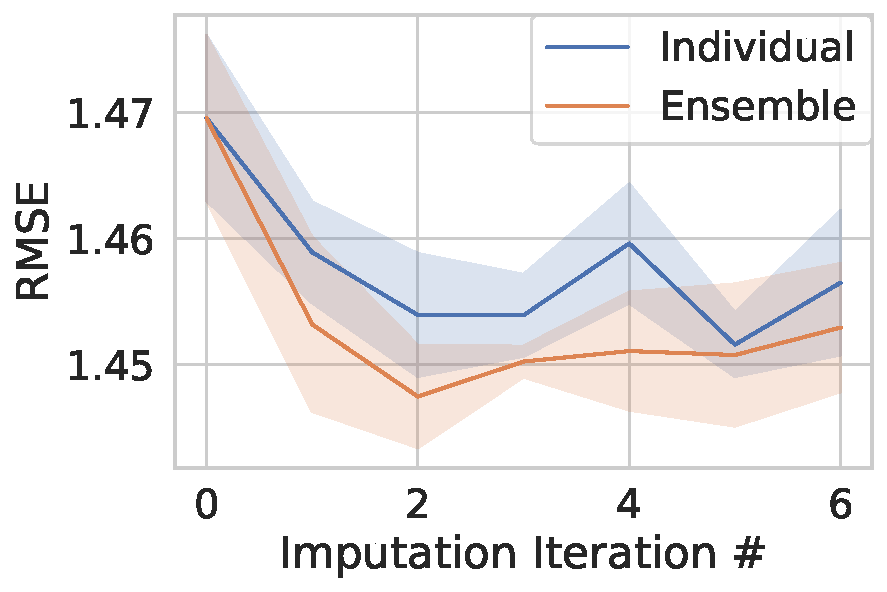
\includegraphics[width=\linewidth]{figures/InitialImpRMSE.pdf}
    \end{subfigure}
    \hfill
    \begin{subfigure}[t]{0.48\textwidth}
        \centering
        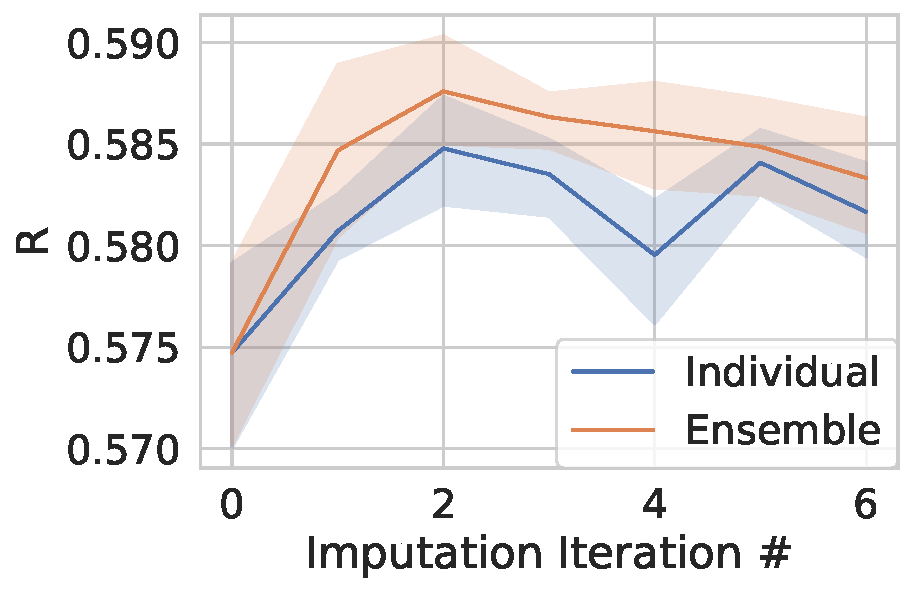
\includegraphics[width=\linewidth]{figures/InitialImpR.pdf}
    \end{subfigure}

    \begin{subfigure}[t]{0.48\textwidth}
        \centering
        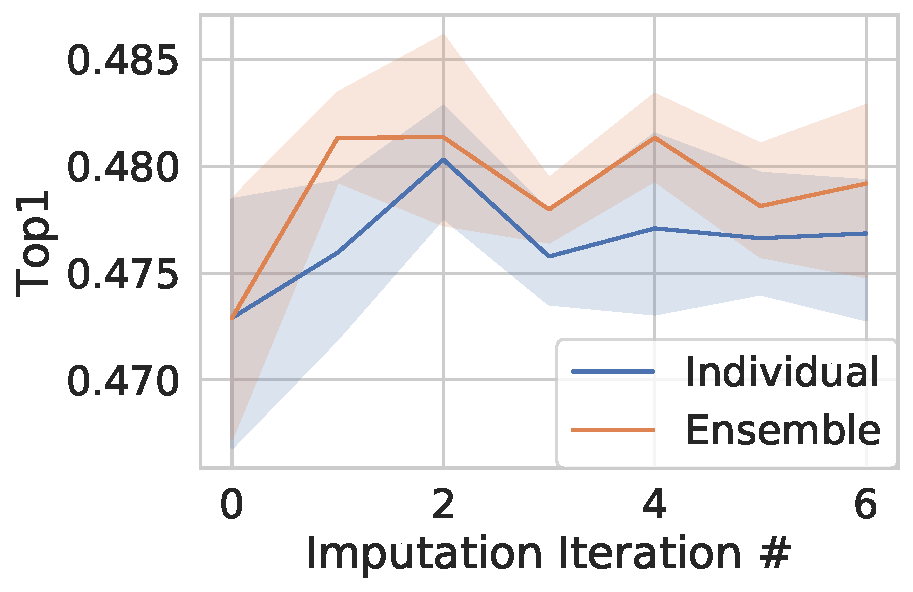
\includegraphics[width=\linewidth]{figures/InitialImpTop1.pdf}
    \end{subfigure}
    \hfill
    \begin{subfigure}[t]{0.48\textwidth}
        \centering
        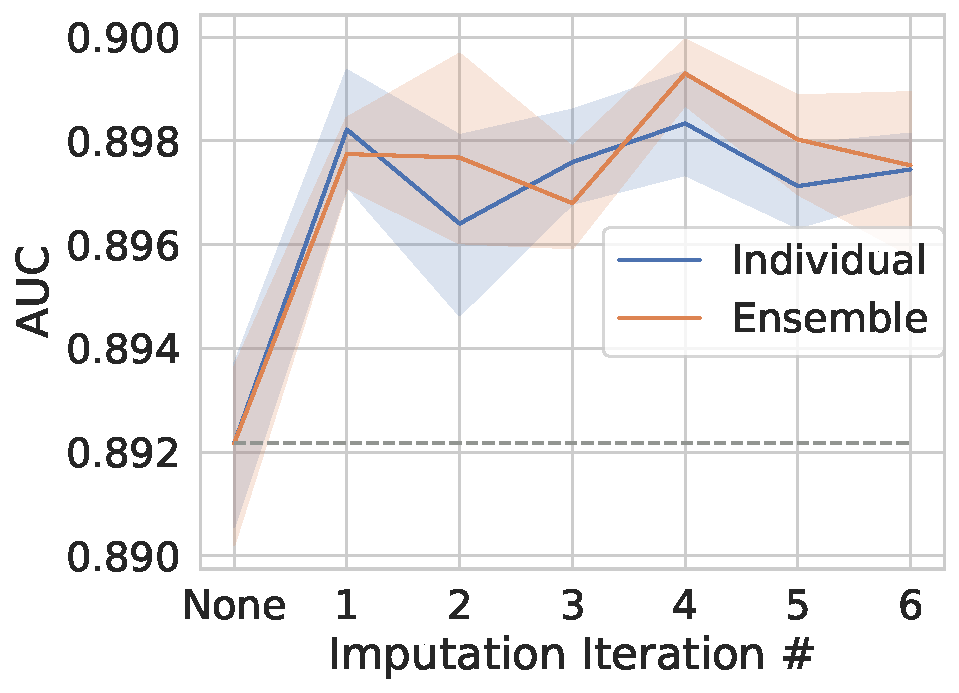
\includegraphics[width=\linewidth]{figures/InitialImpAUC.pdf}
    \end{subfigure}
    \caption{temporary caption}
    \label{fig:initialImp}
\end{figure}





\begin{figure}[tbph]
    \centering
    \begin{subfigure}[t]{0.48\textwidth}
        \centering
        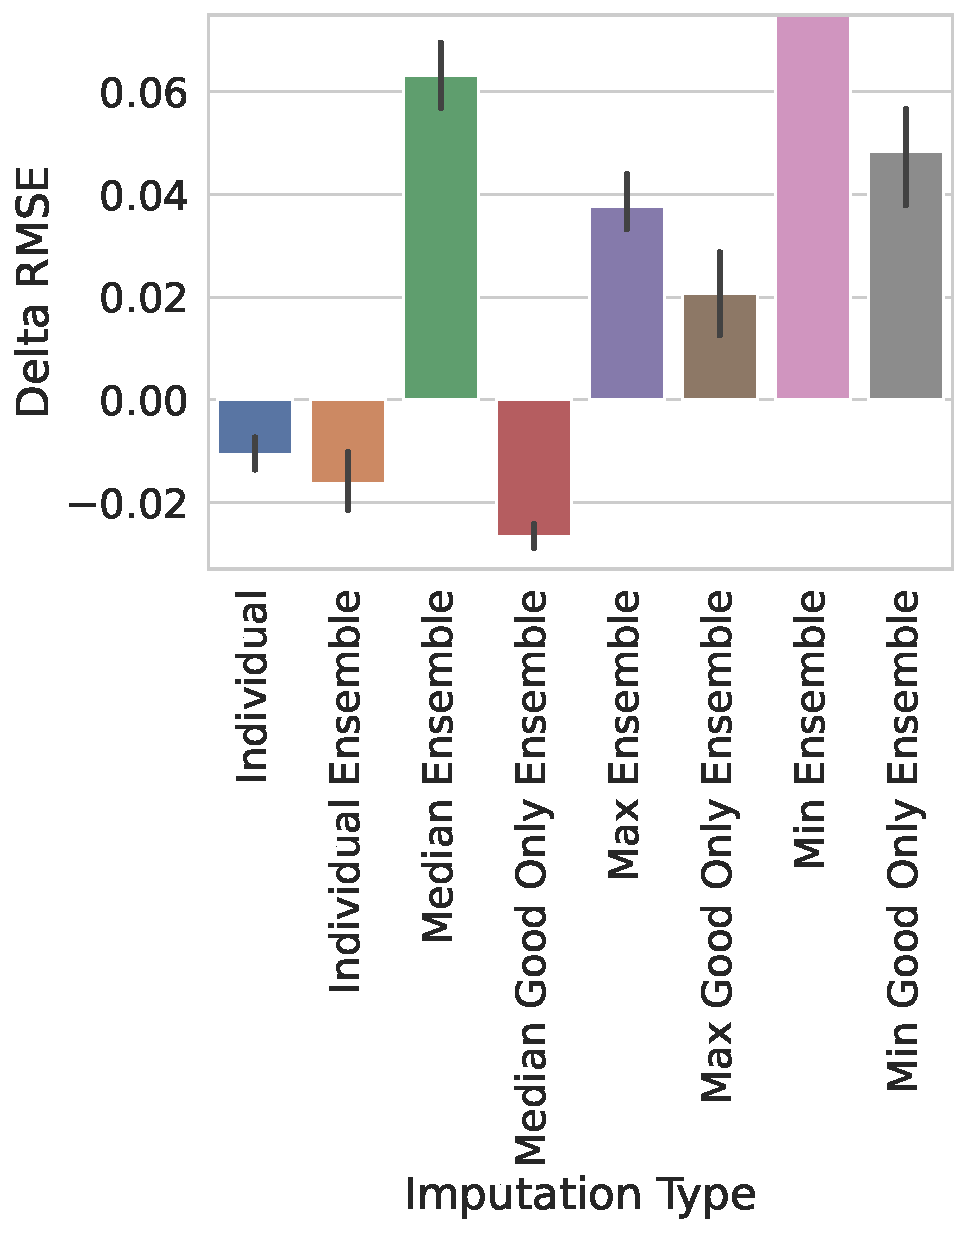
\includegraphics[width=\linewidth]{figures/ComparingImpStylesRMSE.pdf}
    \end{subfigure}
    \hfill
    \begin{subfigure}[t]{0.48\textwidth}
        \centering
        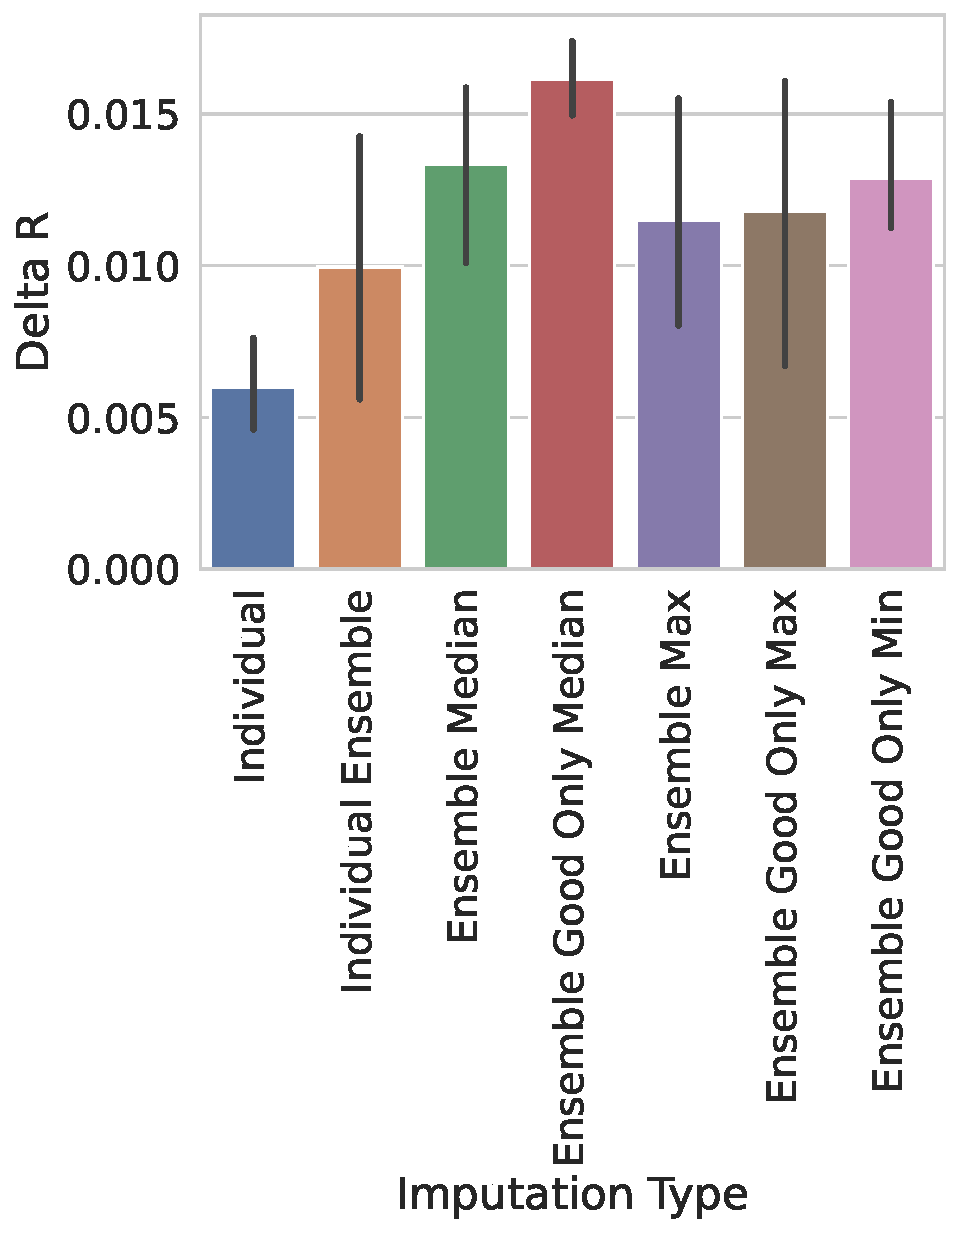
\includegraphics[width=\linewidth]{figures/ComparingImpStylesR.pdf}
    \end{subfigure}

    \begin{subfigure}[t]{0.48\textwidth}
        \centering
        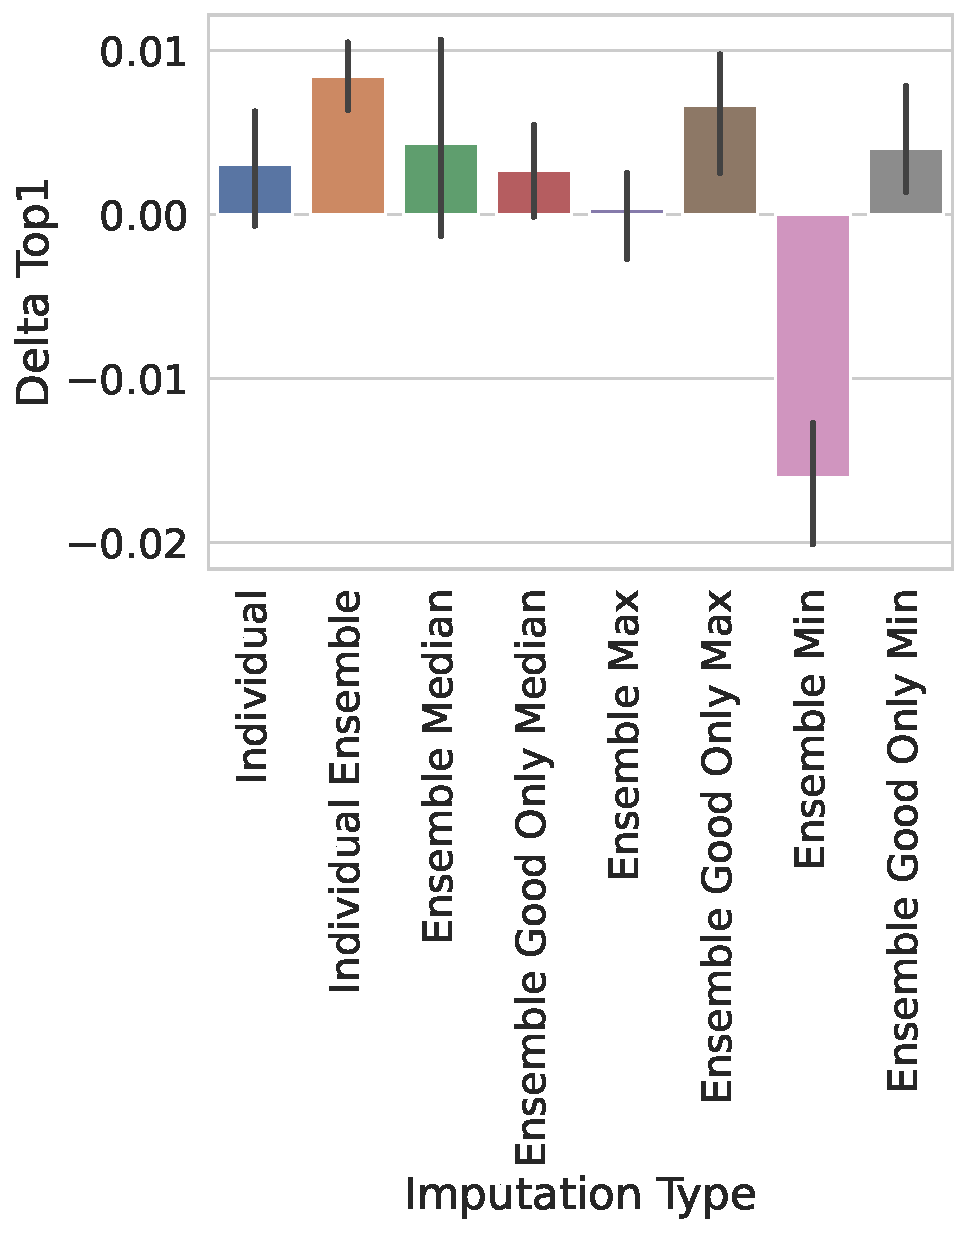
\includegraphics[width=\linewidth]{figures/ComparingImpStylesTop1.pdf}
    \end{subfigure}
    \hfill
    \begin{subfigure}[t]{0.48\textwidth}
        \centering
        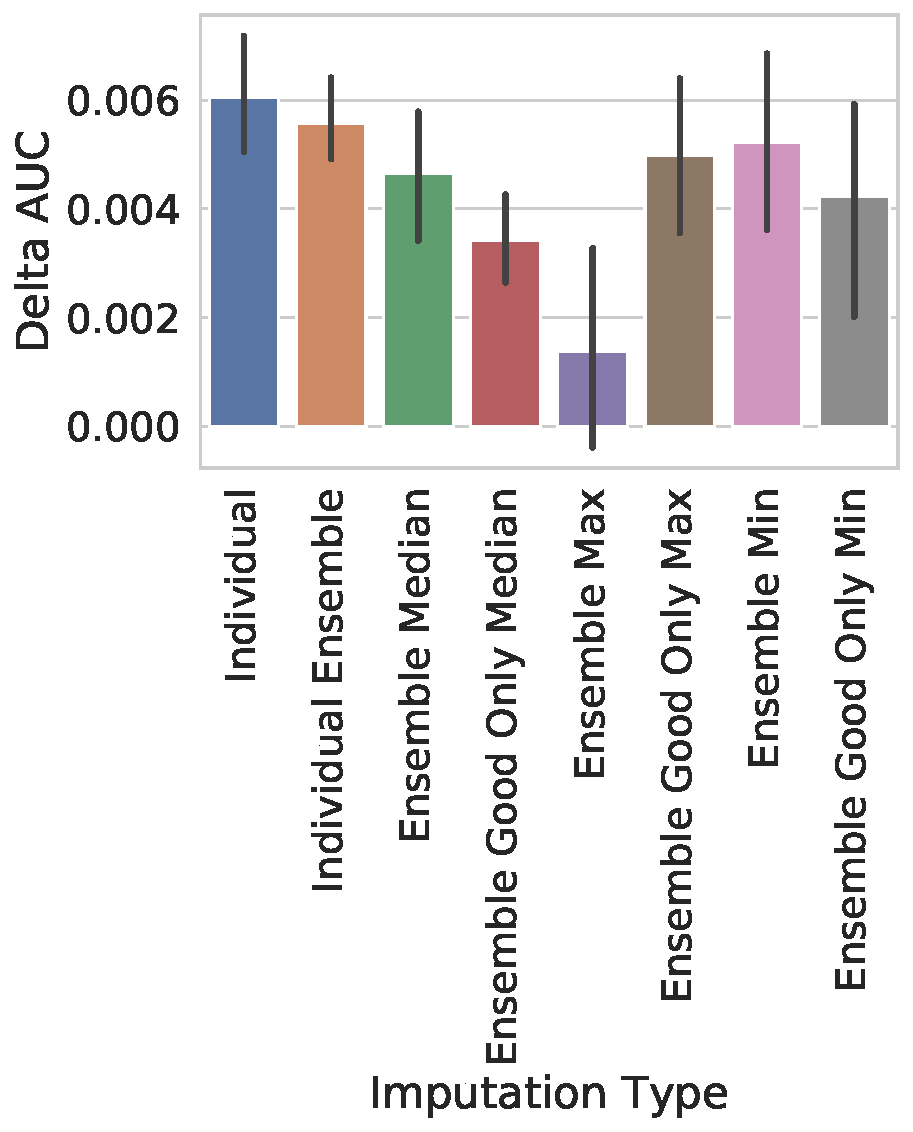
\includegraphics[width=\linewidth]{figures/ComparingImpStylesAUC.pdf}
    \end{subfigure}
    \caption{temporary caption}
    \label{fig:compareImp}
\end{figure}




\begin{figure}[tbph]
    \centering
    \begin{subfigure}[t]{0.48\textwidth}
        \centering
        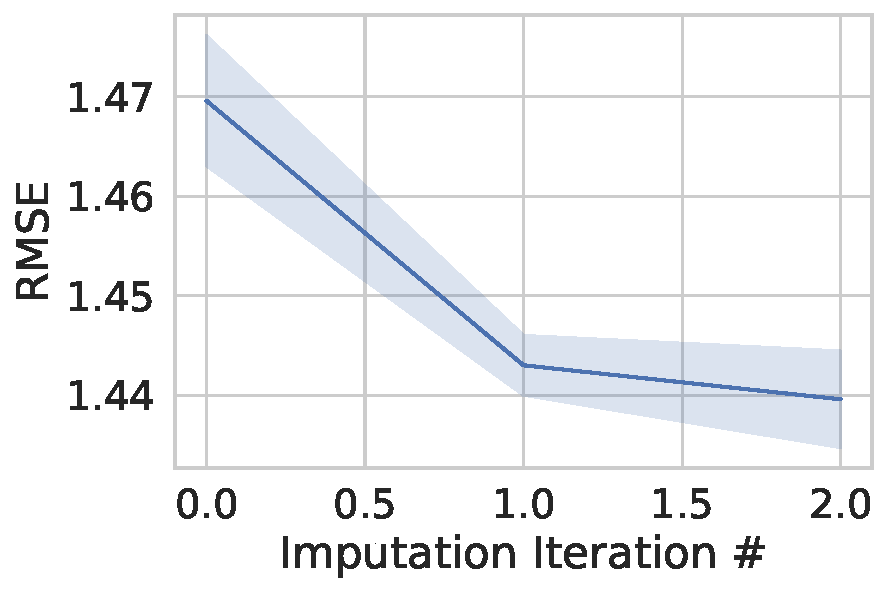
\includegraphics[width=\linewidth]{figures/MedGOEnsRMSE.pdf}
    \end{subfigure}
    \hfill
    \begin{subfigure}[t]{0.48\textwidth}
        \centering
        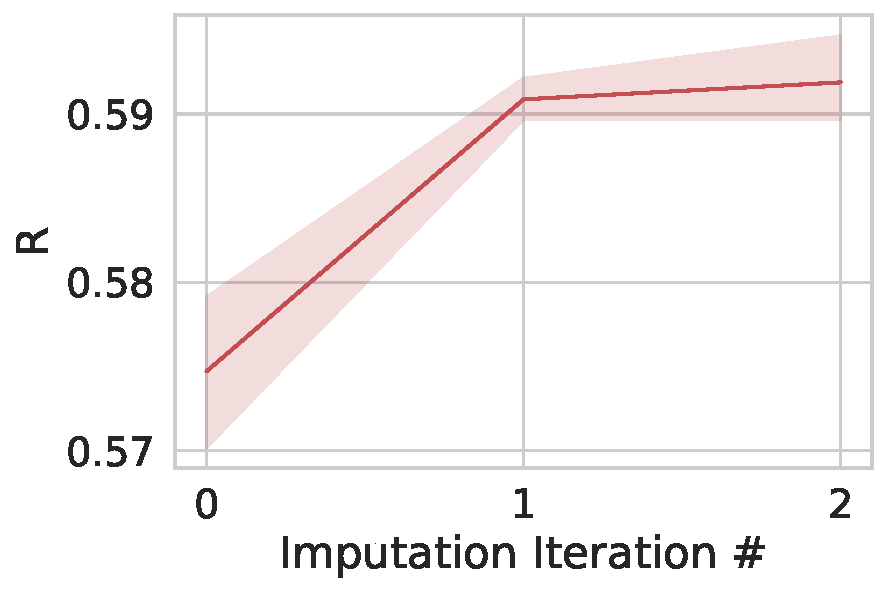
\includegraphics[width=\linewidth]{figures/MedGOEnsR.pdf}
    \end{subfigure}

    \begin{subfigure}[t]{0.48\textwidth}
        \centering
        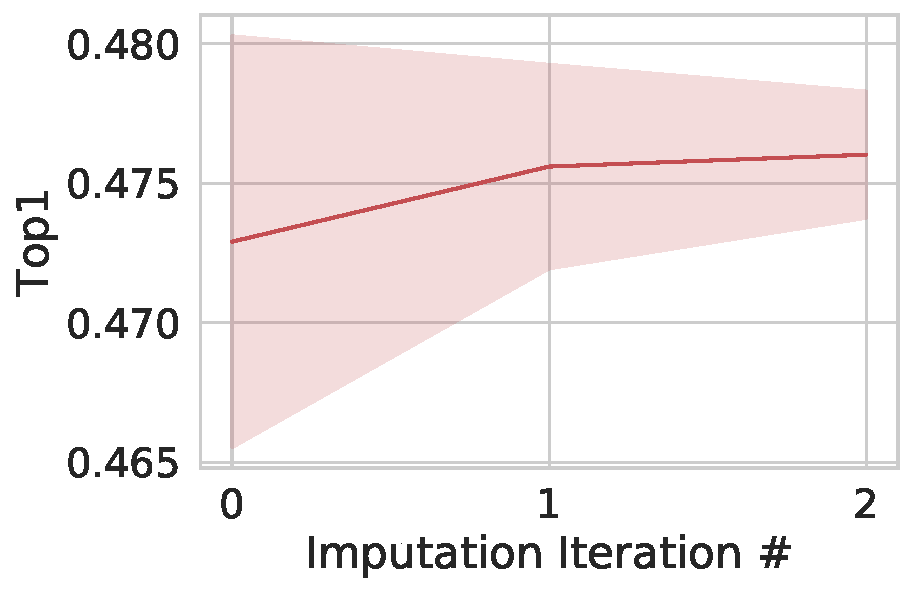
\includegraphics[width=\linewidth]{figures/MedGOEnsTop1.pdf}
    \end{subfigure}
    \hfill
    \begin{subfigure}[t]{0.48\textwidth}
        \centering
        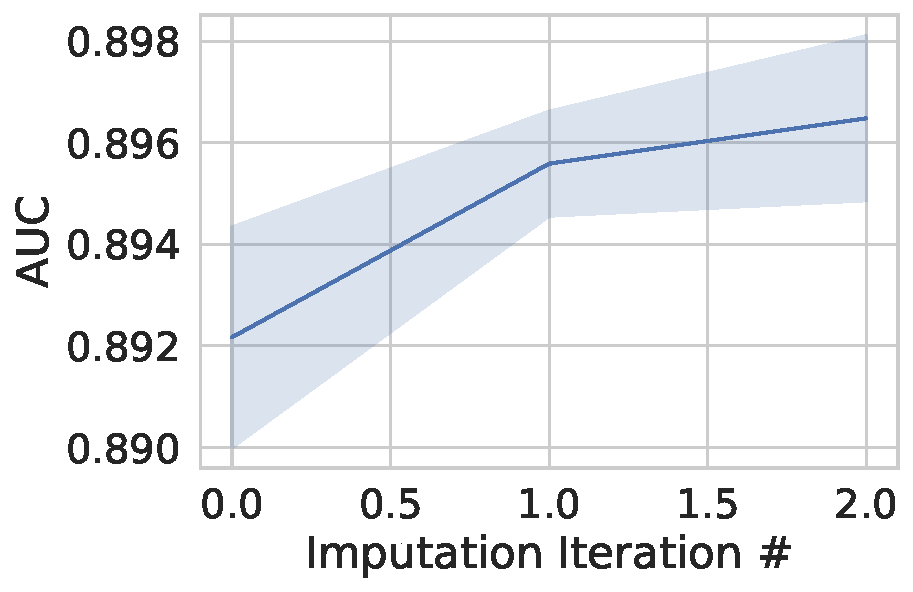
\includegraphics[width=\linewidth]{figures/MedGOEnsAUC.pdf}
    \end{subfigure}
    \caption{temporary caption}
    \label{fig:medGOEnsOverall}
\end{figure}


\begin{figure}[tbph]
    \centering
    \begin{subfigure}[t]{0.48\textwidth}
        \centering
        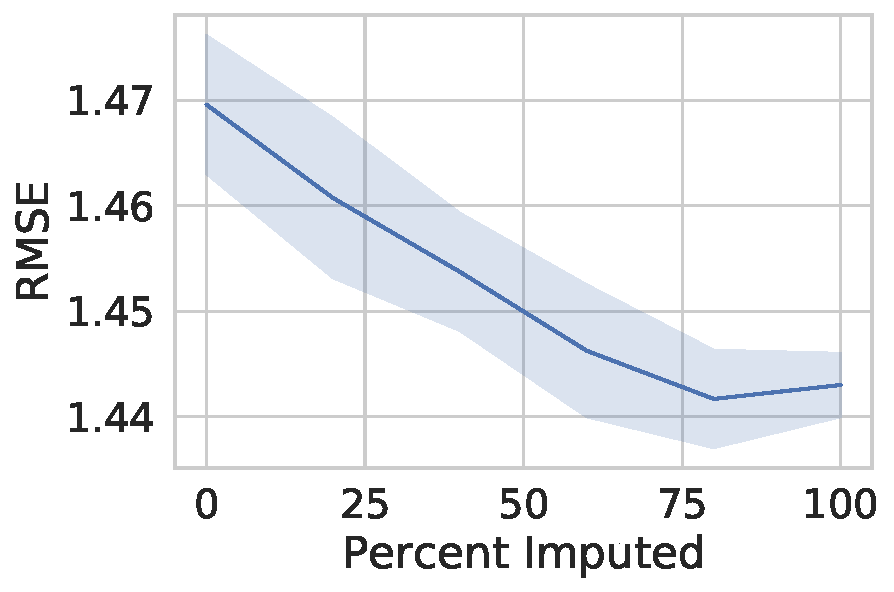
\includegraphics[width=\linewidth]{figures/MedGOEns_addingImpRMSE.pdf}
    \end{subfigure}
    \hfill
    \begin{subfigure}[t]{0.48\textwidth}
        \centering
        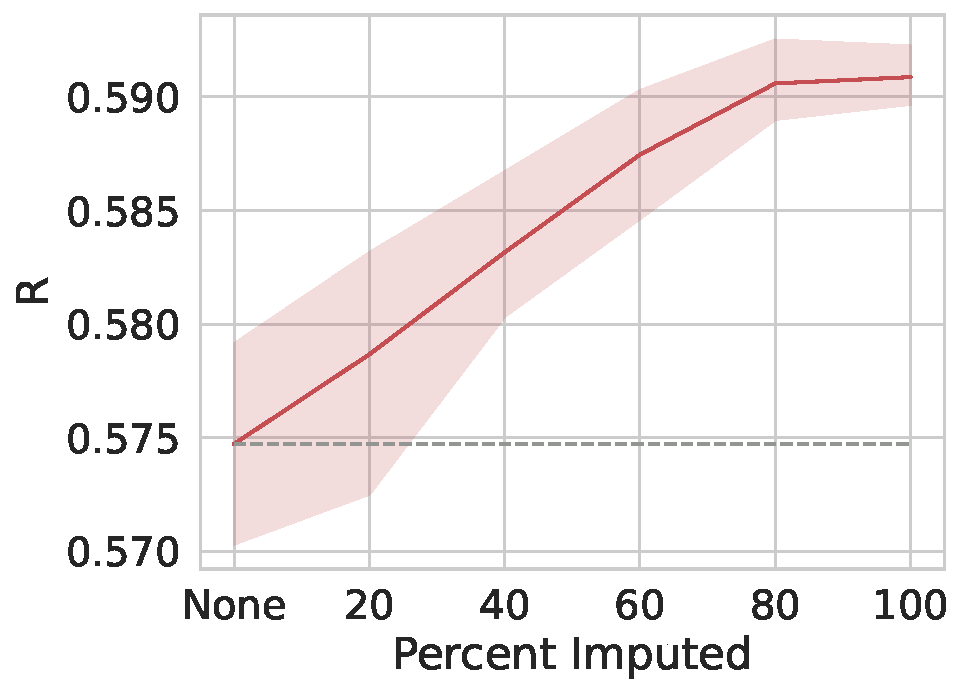
\includegraphics[width=\linewidth]{figures/MedGOEns_addingImpR.pdf}
    \end{subfigure}

    \begin{subfigure}[t]{0.48\textwidth}
        \centering
        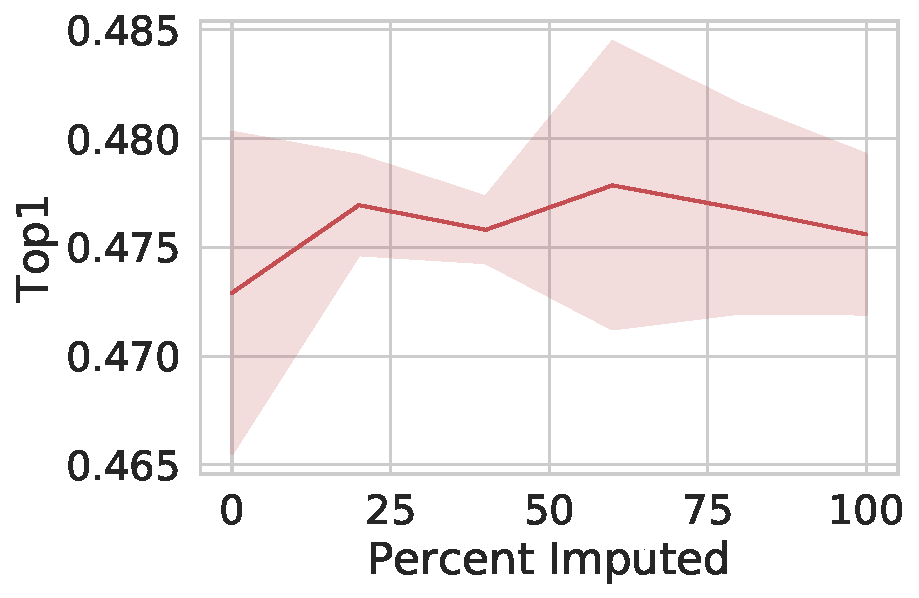
\includegraphics[width=\linewidth]{figures/MedGOEns_addingImpTop1.pdf}
    \end{subfigure}
    \hfill
    \begin{subfigure}[t]{0.48\textwidth}
        \centering
        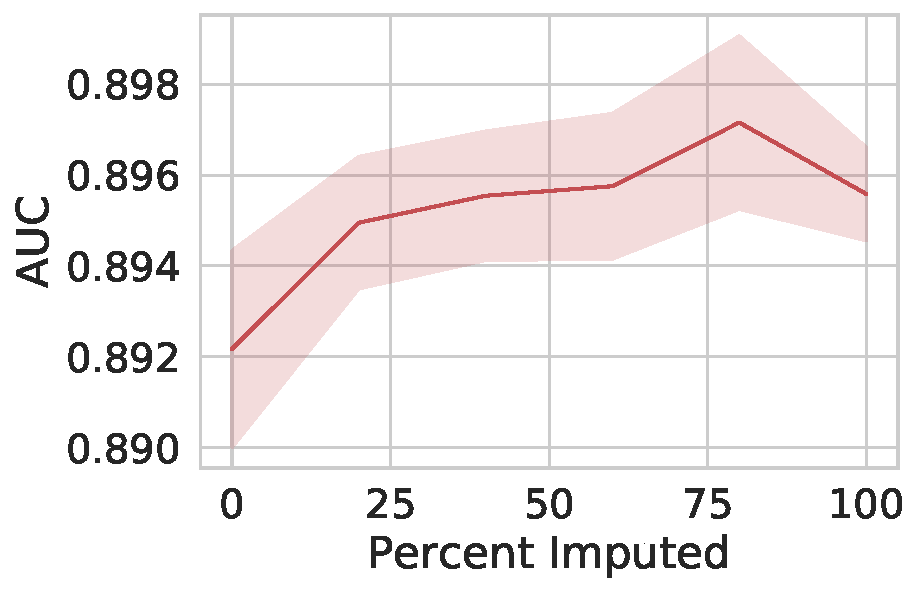
\includegraphics[width=\linewidth]{figures/MedGOEns_addingImpAUC.pdf}
    \end{subfigure}
    \caption{temporary caption}
    \label{fig:medGOEnsAdding}
\end{figure}


\begin{itemize}
    \item Individual vs Ensemble
    \item 1 val for ptn:lig complex
    \item 1 val from GOOD poses for ptn:lig complex
    \item ? scaling the amount of imputation
\end{itemize}

%%%%%%%%%%%%%%%%%%%%%%%%%%%%%%%%%%%%%%%%%%%%%%%%%%%%%%%%%%%%%%%%%%%%%
%% Discussion
%%%%%%%%%%%%%%%%%%%%%%%%%%%%%%%%%%%%%%%%%%%%%%%%%%%%%%%%%%%%%%%%%%%%%
\section{Discussion}
TODO


%%%%%%%%%%%%%%%%%%%%%%%%%%%%%%%%%%%%%%%%%%%%%%%%%%%%%%%%%%%%%%%%%%%%%
%% The "Acknowledgement" section can be given in all manuscript
%% classes.  This should be given within the "acknowledgement"
%% environment, which will make the correct section or running title.
%%%%%%%%%%%%%%%%%%%%%%%%%%%%%%%%%%%%%%%%%%%%%%%%%%%%%%%%%%%%%%%%%%%%%
\begin{acknowledgement}


insert plz

\end{acknowledgement}

%%%%%%%%%%%%%%%%%%%%%%%%%%%%%%%%%%%%%%%%%%%%%%%%%%%%%%%%%%%%%%%%%%%%%
%% The same is true for Supporting Information, which should use the
%% suppinfo environment.
%%%%%%%%%%%%%%%%%%%%%%%%%%%%%%%%%%%%%%%%%%%%%%%%%%%%%%%%%%%%%%%%%%%%%
\begin{suppinfo}

%This will usually read something like: ``Experimental procedures and
%characterization data for all new compounds. The class will
%automatically add a sentence pointing to the information on-line:
%Supporting Information Available: Supplementary Figures (\ref{fig:hyperparamters}-\ref{fig:rotensemble}), Tables (\ref{tab:trainhyper}-\ref{tab:RedCD2020}), and Methods.
\end{suppinfo}

%%%%%%%%%%%%%%%%%%%%%%%%%%%%%%%%%%%%%%%%%%%%%%%%%%%%%%%%%%%%%%%%%%%%%
%% The appropriate \bibliography command should be placed here.
%% Notice that the class file automatically sets \bibliographystyle
%% and also names the section correctly.
%%%%%%%%%%%%%%%%%%%%%%%%%%%%%%%%%%%%%%%%%%%%%%%%%%%%%%%%%%%%%%%%%%%%%
\bibliography{references}

\end{document}